\documentclass[10pt]{article}
\usepackage{multicol}
\usepackage[colorlinks]{hyperref}
\usepackage[czech]{babel}
\usepackage[utf8]{inputenc}
\usepackage[T1]{fontenc}
\usepackage{amsmath}
\usepackage{amsfonts}
\usepackage{amssymb}
\usepackage[version=4]{mhchem}
\usepackage{stmaryrd}
\usepackage{graphicx}
\usepackage[export]{adjustbox}
\graphicspath{ {./images/} }
\usepackage[a4paper, total={6in, 8in},top=2.5cm,bottom=2.5cm]{geometry}

\begin{document}
\section*{Maxwellovy rovnice - připomenutí}
Maxwellovy rovnice nejsou součástí otázek ke zkoušce, ale je dobré si připomenout tento úžasný výtvor.

$$
\begin{aligned}
r o t \vec{H} & =\vec{J}+\frac{\partial \vec{D}}{\partial t} \\
r o t \vec{E} & =-\frac{\partial \vec{B}}{\partial t} \\
\vec{D} & =\varepsilon_{0} \varepsilon_{r} \vec{E} \\
\vec{B} & =\mu_{0} \mu_{r} \vec{H} \\
\vec{J} & =\sigma \vec{E}
\end{aligned}
$$

\section*{1 Elektromagnetická vlna v neohraničeném prostředí}
1.1 Vlnová rovnice pro $\vec{E}$ mimo oblast zdrojů, obecný časový průběh veličin

$$
\Delta \vec{E}-\mu \sigma \frac{\partial \vec{E}}{\partial t}-\mu \varepsilon \frac{\partial^{2} \vec{E}}{\partial t^2}=0
$$

\subsection*{1.2 Vlnová rovnice pro $\hat{\vec{E}}$ (komplexní) mimo oblast zdrojů}
$$
\Delta \hat{\vec{E}}-k^{2} \hat{\vec{E}}=0
$$
$k^{2}=-j \omega \sigma(j \omega \varepsilon+\sigma) \Rightarrow \hat{k}=\sqrt{-j \omega \sigma(j \omega \varepsilon+\sigma)}=\beta-j \alpha$\\
$\mu \ldots$ permeabilita\\
$\varepsilon \ldots$ permitivita\\
$\sigma \ldots$ konduktivita

\subsection*{1.3 Vlnová rovnice pro $\vec{E}$}
Vlnová rovnice pro oblast se zdroji.

$$
\Delta \vec{E}-\mu \varepsilon \frac{\partial^{2}}{\partial t^{2}} \vec{E}-\mu \sigma \frac{\partial \vec{E}}{\partial t}=\mu \frac{\partial j_{m}}{\partial t}+\operatorname{grad} \frac{\rho_{0}}{\varepsilon}
$$

Zdroje vznikají pokud:\\
mění se proudová hustota $\frac{\partial j_{m}}{\partial t}$\\
náboj $\frac{\rho_{0}}{\varepsilon}$ má nějaký gradient\\
1.4 Jak souvisí vektorový potenciál $\vec{A}$ a vektor magnetické indukce $\vec{B}$

$$
\vec{B}=\operatorname{rot} \vec{A}
$$

\subsection*{1.5 Vlnová impedance - definice}
Tady vyloženě chce ten první vztah, vztahy s $\hat k$ jsou pro úplnost \\
$$
\hat{Z}=\frac{\hat{E}_{x}(z)}{\hat{H}_{y}(z)}=\frac{\omega \mu}{\hat{k}}=\frac{\omega \mu}{\sqrt{-j \omega \mu(j \omega \varepsilon+\sigma)}}=\sqrt{\frac{j \omega \mu}{j \omega \varepsilon+\sigma}}
$$
\newpage
\subsection*{1.6 Vlnová impedance vakua - hodnota}
Pokud do rovnice impedance dosadíme hodnoty pro vakuum:\\
$\mu=\mu_{0} \mu_{r}=\mu_{0}$\\
$\varepsilon=\varepsilon_{0} \varepsilon_{r}=\varepsilon_{0}$\\
$\sigma=0 \ldots$ prostředí je nevodivé

$$
Z=\sqrt{\frac{j \omega \mu}{j \omega \varepsilon+\sigma}}=\sqrt{\frac{\mu_{0}}{\varepsilon_{0}}}=120 \pi\text{ } \Omega
$$

\subsection*{1.7 Definujte hloubku vniku vlny}
Charakteristická vzdálenost ve které poklesne amplituda vlny na $1 / e$ (cca $37 \%$).\\
$$
E_{m} e^{-\alpha \cdot z}=E_{m} e^{-1}
$$
Pro takovou vzdálenost plyne:

$$
\alpha z=1 \quad \Rightarrow \quad \delta=\frac{1}{\alpha}
$$
(Velmi často se objevuje v příkladech, vypočíst útlum v nějaké vzdálenosti od rozhraní atd.) \\
POZOR! - Výkon se tlumí z druhou mocninou \\
\subsection*{1.8 Vzorec pro výpočet hloubky vniku vlny do dobrého vodiče}
Z rovnice pro $\hat{k}$ vyjde pro dobrý vodič ( $\omega \varepsilon \ll \sigma$ ):

$$
\alpha=\beta=\sqrt{\frac{\omega \mu \sigma}{2}}
$$
Potom je tedy hloubka vniku $\delta$ rovna:

$$
\delta=\frac{1}{\sqrt{\frac{\omega \mu \sigma}{2}}}
$$

\subsection*{1.9 Vlnová impedance - určení z vlastností prostředí}
Tady chce napsat ten prostřední nebo poslední vztah první není z parametrů prostředí, obsahuje $\hat{k}$
$$
Z=\frac{\omega \mu}{\hat{k}}=\frac{\omega \mu}{\sqrt{-j \omega \mu(j \omega \varepsilon+\sigma)}}=\sqrt{\frac{j \omega \mu}{j \omega \varepsilon+\sigma}}
$$

\subsection*{1.10 Hustota výkonu neseného rovinnou vlnnou - okamžitá hodnota}
$$
\vec{S}=\vec{E} \times \vec{H} \quad\left[\frac{V A}{m^{2}}\right]\left[\frac{V}{m}\right]\left[\frac{A}{m}\right]
$$

\subsection*{1.11 Hustota výkonu neseného rovinnou vlnou ve ztrátovém prostředí - střední časová hodnota}
$$
S_{s t r}(z)=\frac{1}{2} E_{m} e^{-\alpha z} H_{m} e^{-\alpha z} \cos \left(\varphi_{z}\right)=\frac{1}{2} E_{m} H_{m} e^{-{\color{red} 2} \alpha z} \cos \left(\varphi_{z}\right)
$$
\newpage
\subsection*{1.12 Za jakých podmínek dojde složením dvou lineárně polarizovaných vln ke vzniku vlny kruhově polarizované}
Pokud mají stejnou frekvenci a amplitudu, ale fáze jedné z nich je posunutá o $\varphi=90^{\circ}$ a jejich polarizace jsou vzájemně kolmé. Je-li fázový posun obecný, je světlo polarizováno elipticky.\\
\begin{figure}[h!]
    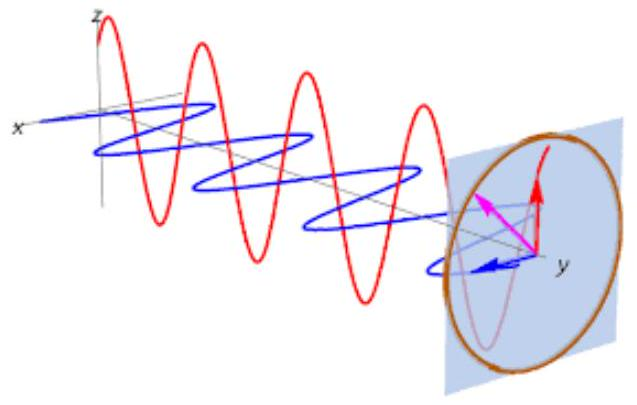
\includegraphics[max width=\textwidth, center]{2025_06_07_aa1708382ad73f838543g-06}
    \caption{Ukázka kruhové polarizace}
\end{figure}


\section*{2 Odraz a lom rovinné vlny}
\subsection*{2.1 Snellův zákon lomu}
Popisuje chování elektromagnetické vlny na rozhraní.

$$
\frac{\sin \vartheta_{I}}{\sin \vartheta_{T}}=\frac{\hat{k}_{I}}{\hat{k}_{T}}=\frac{\sqrt{\varepsilon_{I}}}{\sqrt{\varepsilon_{T}}}
$$
$$
\sin \vartheta_{I} \cdot \sqrt{\varepsilon_{T}} = \sin \vartheta_{T} \cdot \sqrt{\varepsilon_{I}}
$$
kde:\\
$\theta_{I} \ldots$ Úhel pod kterým dopadá vlna na rozhraní\\
$\theta_{R} \ldots$ Úhel pod kterým vlna prostupuje rozhraním\\
$k_{I}, k_{R} \ldots$ Konstanty šíření dopadající/procházející vlny\\
$\varepsilon_{I}, \varepsilon_{R} \ldots$ Relativní permitivity prostředí kterým vlna prochází\\
\\
Zároveň říká, že úhel dopadu a odrazu je shodný
\newpage
\subsection*{2.2 Definujte rovinu dopadu}
Referenční rovina od které odvozujeme polarizace. Zpravidla se jedná o rovinu xz.\\

\begin{figure}[h!]
    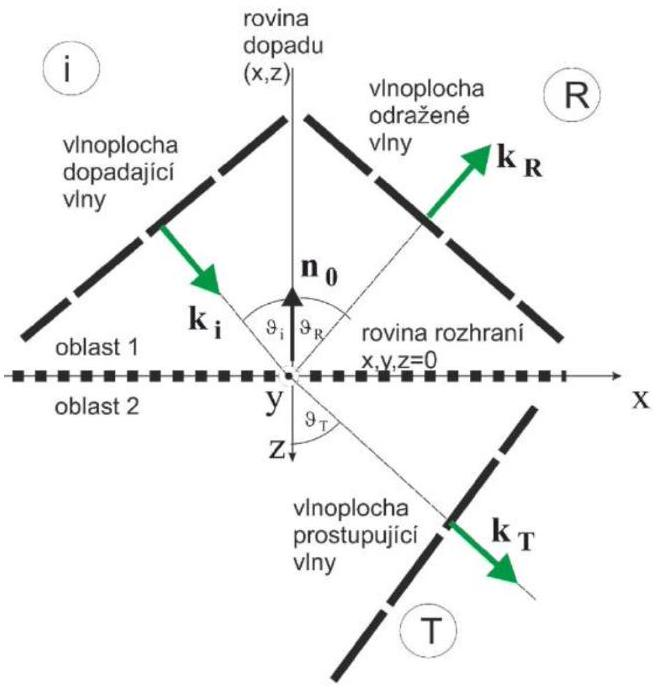
\includegraphics[max width=(\textwidth/3), center]{2025_06_07_aa1708382ad73f838543g-07(2)}
    \caption{Ukázka rozhraní na které dopadá vlna}
\end{figure}

\subsection*{2.3 Zakreslete vektory $\vec{E}, \vec{H}, \vec{S}$ do roviny dopadu pro případ rovnoběžné a kolmé polarizace dopadající vlny}
\section*{Spojené dvě otázky}
\begin{itemize}
  \item Rovnoběžná polarizace - vektor elektrické složky je rovnoběžný s rovinou dopadu (rovina xz, resp. rovina papíru).
  \item Kolmá polarizace - vektor je kolmý na rovinu dopadu.
\end{itemize}

\begin{figure}[h!]
\centering
\begin{minipage}[t]{0.48\textwidth}
    \centering
    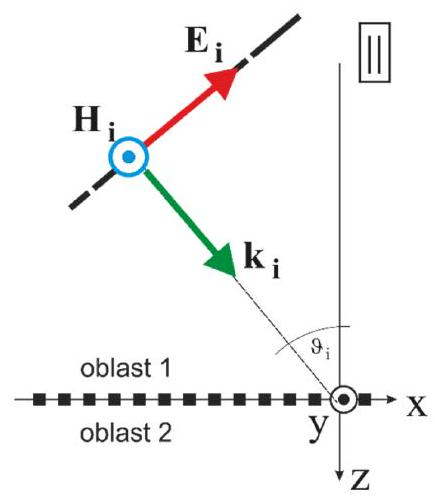
\includegraphics[width=\textwidth]{2025_06_07_aa1708382ad73f838543g-07}
    \caption{ Rovnoběžná polarizace}
\end{minipage}
\hfill
\begin{minipage}[t]{0.48\textwidth}
    \centering
    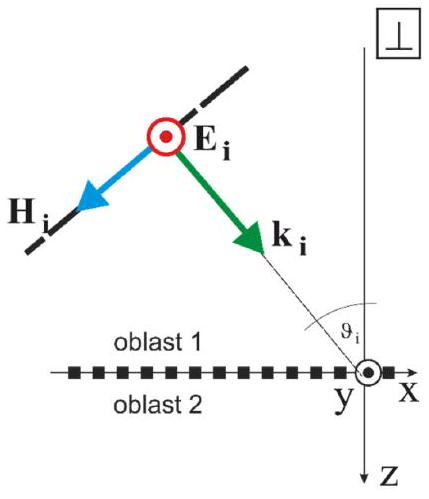
\includegraphics[width=\textwidth]{2025_06_07_aa1708382ad73f838543g-07(1)}
    \caption{ Kolmá polarizace}
\end{minipage}
\end{figure}

\newpage

\subsection*{2.5 Co je mezní úhel a jak závisí na permitivitě při odrazu vlny na rozhraní dvou dielektrik}
Úlhel dopadající vlny při kterém se úhel lomu rovná $90^{\circ}$, celá vlna tedy potuje rozhraním. Objevuje se pokud vlna prochází z elektricky hustšího prostředí do elektricky řidšího $\left(\varepsilon_{r 2}<\varepsilon_{r 1}\right)$.

$$
\sin \theta_{1}=\frac{k_{I} \cdot \sin \theta_{2}}{k_{R}} \quad \stackrel{\theta_{2}=\frac{\pi}{2}}{\Longrightarrow} \quad \sin \theta_{1}=\frac{k_{I}}{k_{R}} \quad \Rightarrow \quad \theta_{1}=\arcsin \left(\frac{k_{I}}{k_{R}}\right)=\arcsin \left(\sqrt{\frac{\varepsilon_{2}}{\varepsilon_{1}}}\right)
$$

\subsection*{2.6 Na rozhraní prostředí s permitivitami $\varepsilon_{r1} > \varepsilon_{r2}$ dochází k totálnímu odrazu elektromagnetické vlny. Zakreslete plochy konstantní fáze a konstantní amplitudy pro vlny na obou stranách rozhraní}

Lepší obrázky jsem nikde nenašel, ale jde o to, že v řidším prostředí se šíří evanescentní vlna, které klesá amplituda čím dál je od rozhraní (roviny konstantních amplitud budou rovnoběžné s rovinou rozhraní). Roviny konstantní fáze jsou pak kolmé na rozhraní. Nad rozhraním, v elektricky hustším prostředí, je stojaté vlnění – tj. roviny konstantní amplitudy a fáze by měly tvořit takové kmitající shluky.

\begin{figure}[h!]
\centering
\begin{minipage}[t]{0.48\textwidth}
    \centering
    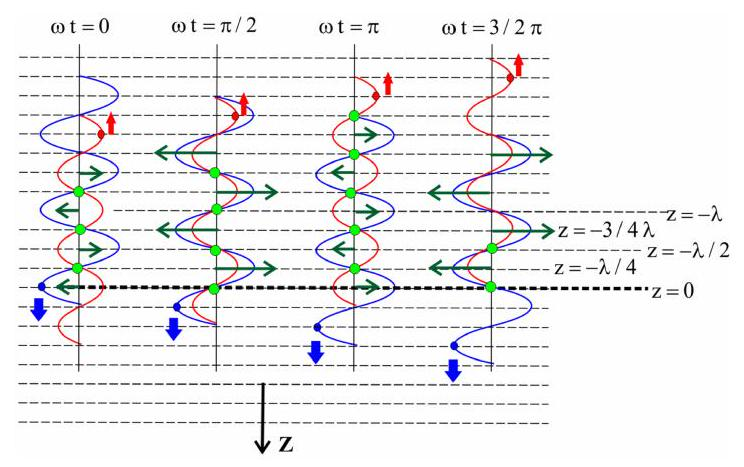
\includegraphics[width=\textwidth]{2025_06_07_aa1708382ad73f838543g-08(1)}
    \caption{Stojaté vlnění – roviny konstantní amplitudy a fáze}
\end{minipage}
\hfill
\begin{minipage}[t]{0.48\textwidth}
    \centering
    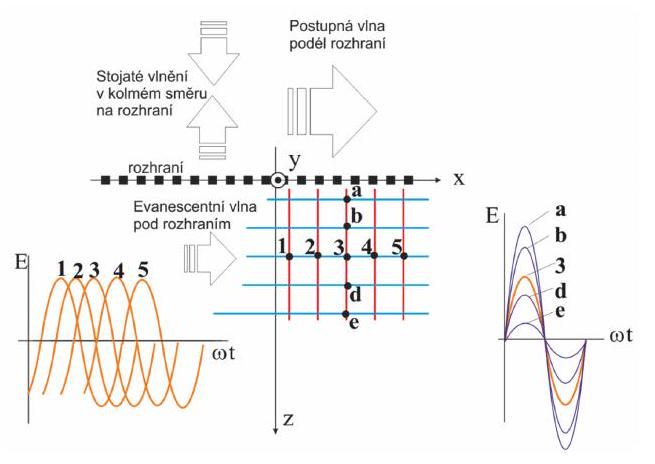
\includegraphics[width=\textwidth]{2025_06_07_aa1708382ad73f838543g-08}
    \caption{Evanescentní vlna – amplitudy a fáze pod rozhraním}
\end{minipage}
\end{figure}

\subsection*{2.7 Co je Brewsterův úhel a jak se určí z vlastností prostředí pro rovnoběžnou polarizaci}

Hledáme úhel dopadu elektromagnetické vlny na rozhraní dvou dielektrik takový, aby činitel odrazu pro rovnoběžně polarizovanou složku byl nulový. Pro rovnoběžně polarizovatelnou složku takový úhel reálně existuje a lze jej spočítat pomocí následujícího vztahu:

\[
\tan \theta_B = \frac{n_2}{n_1}
\]

kde:
- $\theta_B$ je Brewsterův úhel,
- $n_1$, $n_2$ jsou indexy lomu prostředí ($n = \sqrt{\varepsilon_r}$).


$$
\theta_{i-B r}=\arcsin \sqrt{\frac{\varepsilon_{r 2}}{\varepsilon_{r 1}+\varepsilon_{r 2}}}=\arcsin \frac{1}{\sqrt{1+\frac{\varepsilon_{r 1}}{\varepsilon_{r 2}}}}
$$

Tento úhel lze využít například na filtrování jedné polarizace z obecného světla. Rovnice byla odvozená pro nemagnetická dielektrika $\left(\mu_{r 1}=\mu_{r 2}=1\right)$
\newpage
\subsection*{2.8 Co je Brewsterův úhel a jak se určí z vlastností prostředí pro kolmou polarizaci}
Matematicky lze spočítat avšak realizovat jej je prakticky nemožné. V tomto případě musí si být rovné permitivity materiálů na rozhraní a pro permeability musí být splněna následující podmínka:

$$
\theta_{i-B r}=\arcsin \sqrt{\frac{\mu_{r 2}}{\mu_{r 1}+\mu_{r 2}}}=\arcsin \frac{1}{\sqrt{1+\frac{\mu_{r 1}}{\mu_{r 2}}}}
$$

\subsection*{2.9 Kolik procent výkonu se odrazí od povrchu dielektrika při kolmém dopadu vlny z vakua o permitivitě dielektrika $\varepsilon_{r}=4$}
Použiji vzorec pro výpočet činitele odrazu.

$$
\hat{R}=\frac{\hat{Z}_{2}-\hat{Z}_{1}}{\hat{Z}_{2}+\hat{Z}_{1}}=\frac{\frac{120}{\sqrt{\varepsilon_{r 2}}}-\frac{120}{\sqrt{\varepsilon_{r 1}}}}{\frac{120}{\sqrt{\varepsilon_{r 2}}}+\frac{120}{\sqrt{\varepsilon_{r 1}}}}=\frac{\sqrt{\varepsilon_{r 1}}-\sqrt{\varepsilon_{r 2}}}{\sqrt{\varepsilon_{r 1}}+\sqrt{\varepsilon_{r 2}}}
$$

Po dosazení $\varepsilon_{r 2}=4$ a $\varepsilon_{r 1}=1$ dostanu výsledek:\\
$\hat{R}=-1 / 3$, odrazí se $11 \%$ výkonu (výkon je $E_{R m}^{2}=E_{I m}^{2}|R|^{2} \Rightarrow$ odrazí se $1 / 9$ výkonu). Zároveň se otočí fáze o $\pi$.

\section*{3 Vedené vlny}
\subsection*{3.1 Definujte vlnu TEM}
Vlna ve které se složka intenzity elektrického pole a magnetického pole šíří kolmo na sebe a zároveň kolmo na směr šíření. Typické je pro koaxiální kabely.\\
T. . . Transverzální, kolmý\\
E. . . Veličiny elektrického pole jsou kolmé na směr šíření\\
M. . Veličiny magnetického pole jsou kolmé na směr šíření

\subsection*{3.2 Definujte vlnu TE}
Složka intenzity elektrického pole je v rovině kolmé na směr šíření, intenzita magnetického pole omezena není, může být i ve směru šíření. Typické pro vlnovody.\\
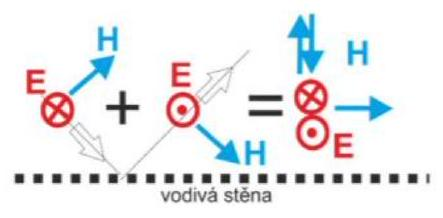
\includegraphics[max width=\textwidth, center]{2025_06_07_aa1708382ad73f838543g-09}

Obrázek 5: Mód TE

\subsection*{3.3 Definujte vlnu TM}
Složka intenzity magnetického pole je vždy kolmá na směr šíření, intenzita elektrického pole žádné omezení nemá, může mířit i ve směru šíření. Typické pro vlnovody.\\
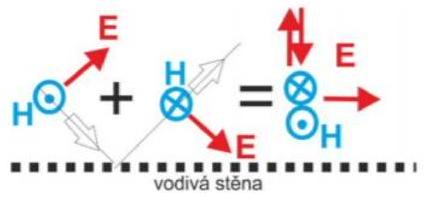
\includegraphics[max width=\textwidth, center]{2025_06_07_aa1708382ad73f838543g-10}

Obrázek 6: Mód TM

\subsection*{3.4 Definujte charakteristickou impedanci vedení}
Charakteristická impedance vedení udává poměr fázorů příslušných napětových a proudových složek na vedení.

$$
\hat{Z}_{0}=\frac{\hat{U}_{+}(z)}{\hat{I}_{+}(z)}=\frac{\hat{U}_{-}(z)}{\hat{I}_{-}(z)}=\sqrt{\frac{R+j \omega \cdot L}{G+j \omega \cdot C}}
$$

Pro bezeztrátové vedení platí:

$$
R=0, G=0 \quad Z_{0}=\sqrt{\frac{L}{C}}
$$

\subsection*{3.5 Telegrafní rovnice pro harmonický časový průběh veličin}
Tady moc nevím jaký tvar přesně chce, ale v žádné teoretické části se na ni nezeptal, takže to je asi stejně jedno. Dávám sem proto nějaký tvar telegrafní rovnice z wiki.

$$
\begin{aligned}
\frac{\partial}{\partial x} \vec{V}_{\omega}(x) & =-\left(j \omega L_{\omega+R_{\omega}}\right) \vec{I}_{\omega}(x) \\
\frac{\partial}{\partial x} \vec{I}_{\omega}(x) & =-\left(j \omega C_{\omega+G_{\omega}}\right) \vec{V}_{\omega}(x)
\end{aligned}
$$

\subsection*{3.6 Uved'te vztah pro výpočet charakteristické impedance (bezeztrátového)}
 koaxiálního vedení$$
R=0, G=0 \quad Z_{0}=\sqrt{\frac{L}{C}} \quad Z_{0}=\frac{60}{\sqrt{\varepsilon_{r}}} \ln \left(\frac{b}{a}\right)
$$

Poslední rovnice je pro výpočet z parametrů prostředí.

\subsection*{3.7 Jaká je kritická frekvence koaxiálního vedení}
$$
f_{k r i t}=\frac{c}{a \pi \sqrt{\varepsilon_{r}}}\left(\frac{1}{1+b / a}\right)
$$

\subsection*{3.8 Nakreslete rozložení (siločáry) $\vec{E}$ a $\vec{H}$ dominantního modu v průřezu koaxiálního vedení}

\begin{figure}[h!]
\centering
\begin{minipage}[t]{0.48\textwidth}
    \centering
    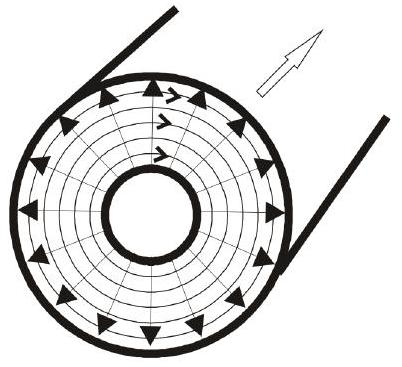
\includegraphics[width=\textwidth]{2025_06_07_aa1708382ad73f838543g-11(2)}
    \caption{Koaxiální kabel – $\vec{E}$ radiálně, $\vec{H}$ soustředně}
\end{minipage}
\hfill
\begin{minipage}[t]{0.48\textwidth}
    \centering
    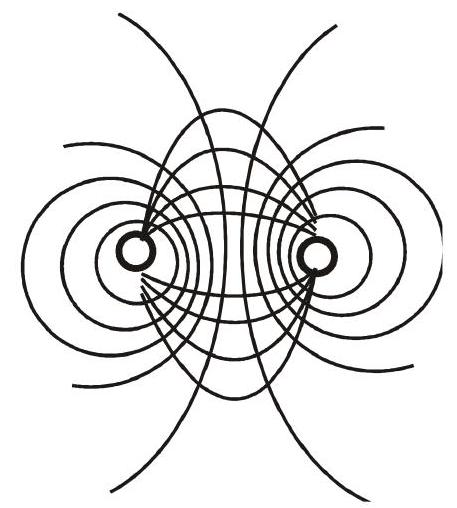
\includegraphics[width=\textwidth]{2025_06_07_aa1708382ad73f838543g-11(1)}
    \caption{Symetrická dvojlinka – siločáry $\vec{E}$ a $\vec{H}$}
\end{minipage}
\end{figure}

\subsection*{3.9 Uved'te kritickou frekvenci dominantního modu vlnovodu s kovovými stěnami obdélníkového průřezu s delší stranou $a$}
Dominantní mód je první mód, který už povede vlnu.\\
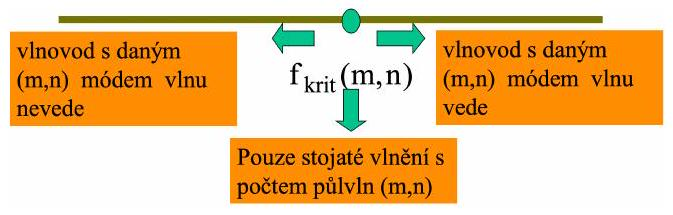
\includegraphics[max width=\textwidth, center]{2025_06_07_aa1708382ad73f838543g-11}

Pro obecný mód ( $\mathrm{m}, \mathrm{n}$ ):

$$
f_{k r i t(m, n)}=\frac{c}{2 \pi \sqrt{\varepsilon_{r}}} \sqrt{\left(\frac{m \cdot \pi}{a}\right)^{2}+\left(\frac{n \cdot \pi}{b}\right)^{2}}=\frac{c}{2 \sqrt{\varepsilon_{r}}} \sqrt{\left(\frac{m}{a}\right)^{2}+\left(\frac{n}{b}\right)^{2}}
$$

Pro první dominantní mód $\mathrm{TE}_{10}$ :

$$
f_{k r i t(m=1, n=0)}=\frac{c}{2 a \sqrt{\varepsilon_{r}}}
$$
\newpage
\subsection*{3.10 Vzorec pro určení vlnové délky dominantního modu vlnovodu s kovovými stěnami obdélníkového průřezu s delší stranou $a$}
Vychází z kritické frekvence vypočítané v části 3.9

$$
\lambda=\frac{2 \pi}{k_{z}}=\frac{c}{\sqrt{\varepsilon_{r}}} \frac{1}{\sqrt{f^{2}-f_{k r i t(m, n)}^{2}}}
$$

Ve skriptech se jedná o vztah 3.14
\subsection*{3.11 Nakreslete rozložení (siločáry) $\vec{E}$ a $\vec{H}$ dominantního modu v průřezu vlnovodu s kovovými stěnami obdélníkového průřezu}

Na následujících obrázcích je několik ukázek možností módů ve vlnovodech.

\begin{figure}[h!]
\centering
\begin{minipage}[t]{0.49\textwidth}
    \centering
    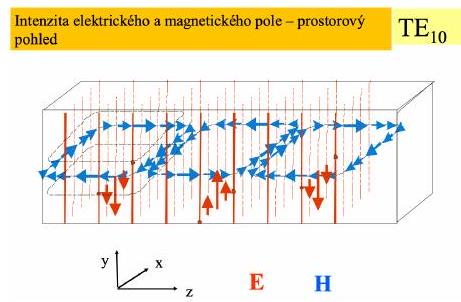
\includegraphics[width=\textwidth]{2025_06_07_aa1708382ad73f838543g-12(1)}
    \caption{Ukázka intenzity $\vec{E}$ a $\vec{H}$ pro mód $\mathrm{TE}_{10}$}
\end{minipage}
\hfill
\begin{minipage}[t]{0.49\textwidth}
    \centering
    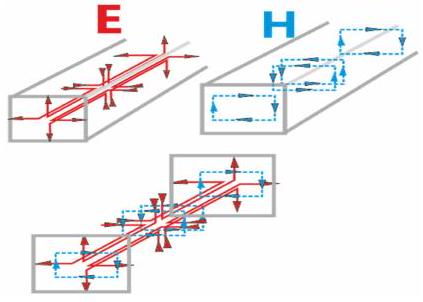
\includegraphics[width=\textwidth]{2025_06_07_aa1708382ad73f838543g-12(2)}
    \caption{Vlna $\mathrm{TM}_{11}$}
\end{minipage}
\end{figure}

\begin{figure}[h!]
\centering
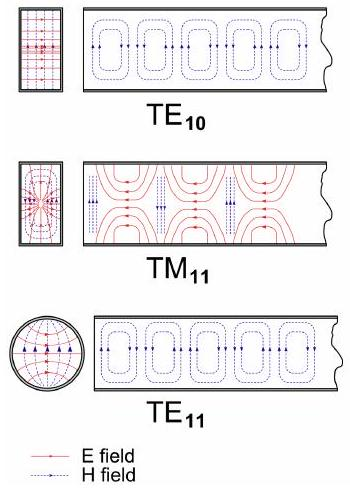
\includegraphics[width=0.4\textwidth]{2025_06_07_aa1708382ad73f838543g-12}
\caption{Další módy pro lepší představu}
\end{figure}


\newpage

\subsection*{3.12 Vzorec pro určení fázové rychlosti šíření dominantního modu vlnovodu s kovovými stěnami obdélníkového průřezu s delší stranou $a$}
Opět je uvedena kritická frekvence ze sekce 3.9

$$
v_{f}=\frac{\omega}{k_{z}}=\frac{c}{\sqrt{\varepsilon_{r}}} \frac{1}{\sqrt{1-\left(\frac{f_{k r i t(m, n)}}{f}\right)^{2}}}
$$

Ve skriptech se jedná o vztah 3.15\\
3.13 Vzorec pro určení skupinové rychlosti šíření dominantního modu vlnovodu s kovovými stěnami obdélníkového průřezu s delší stranou $a$

$$
v_{s k}=\frac{d \omega}{d k_{z}}=\frac{c}{\sqrt{\varepsilon_{r}}} \frac{\sqrt{\omega^{2}-\left(2 \pi f_{k r i t(m, n))^{2}}\right.}}{\omega}=\frac{c}{\sqrt{\varepsilon_{r}}} \sqrt{1-\left(\frac{f_{k r i t(m, n)}}{f}\right)^{2}}
$$

Ve skriptech se jedná o vztah 3.16

\subsection*{3.14 Vzorec pro určení vlnové impedance dominantního modu vlnovodu s kovovými stěnami obdélníkového prữezu s delší stranou $a$}
Pro TE:

$$
\frac{\hat{E}_{x}}{\hat{H}_{y}}=-\frac{\hat{E}_{y}}{\hat{H}_{x}}=\frac{\omega \mu}{k_{z}}=Z_{T E}
$$

Ve skriptech vztah 3.55

\subsection*{3.15 Uved'te kritickou frekvenci nejnižšího TM modu vlnovodu s kovovými stěnami obdélníkového průřezu s rozměry $\mathrm{a} \times \mathrm{b}$}
$$
f_{k r i t(m, n)}=\frac{c}{2 \pi \sqrt{\varepsilon_{r}}} \sqrt{\left(\frac{m \cdot \pi}{a}\right)^{2}+\left(\frac{n \cdot \pi}{b}\right)^{2}}=\frac{c}{2 \sqrt{\varepsilon_{r}}} \sqrt{\left(\frac{m}{a}\right)^{2}+\left(\frac{n}{b}\right)^{2}}
$$

\subsection*{3.16 Uved'te vlnovou impedanci nejnižšího TM modu vlnovodu s kovovými stěnami obdélníkového průřezu s rozměry $\mathrm{a} \times \mathrm{b}$}

Pro TM:

$$
\frac{\hat{E}_{x}}{\hat{H}_{y}}=-\frac{\hat{E}_{y}}{\hat{H}_{x}}=\frac{k_{z}}{\omega \varepsilon}=Z_{T M}
$$

Ve skriptech vztah 3.37\\
\subsection*{3.17 Uved'te vztah pro maximální střední časovou hodnotu výkonu přenášeného vlnovodem s kovovými stěnami obdélníkového průřezu s rozměry a x b při elektrické pevnosti dielektrika $E_{\text {max }}$}

$$
P=\frac{a b}{4} \frac{E_{\max }^{2}}{Z_{T E}}
$$

Ve skriptech vztah 3.72

\subsection*{3.18 Vztah pro určení rezonančních frekvencí dutinového rezonátoru ve tvaru kvádru s kovovými stěnami a vnitřními rozměry a x b x c}
Matematický popis je velice podobný obdélníkovému vlnovodu. K číslům $m$ a $n$ přibude ještě další číslo $p$, které značí počet půlvln stojatého vlnění v ose z.

$$
f_{r e z}=\frac{c}{2 \pi \sqrt{\varepsilon_{r}}} \sqrt{\left(\frac{m \cdot \pi}{a}\right)^{2}+\left(\frac{n \cdot \pi}{b}\right)^{2}+\left(\frac{p \cdot \pi}{l}\right)}=\frac{c}{2 \sqrt{\varepsilon_{r}}} \sqrt{\left(\frac{m}{a}\right)^{2}+\left(\frac{n}{b}\right)^{2}+\left(\frac{p}{l}\right)^{2}}
$$

Ve skriptech vztah 3.73

\section*{4 Vyzařování vln}
\subsection*{4.1 Co je vyzařovací charakteristika (antény)}
Grafické znázornění směrového vyzařování elektromagnetické energie antény do prostoru. Obvykle je zobrazena ve 2 D ve formě polárního nebo xy grafu, případně ve 3 D . Vyzařovací charakteristika antény závisí na jejím tvaru, velikosti, konstrukci materiálu a pracovní frekvenci

\subsection*{4.2 Vyzařovací charakteristika elementárního dipólu}
Elementární dipól vyzařuje do v horizontálním směru na všechny strany stejně (obrázek nalevo). Ve vertikálním směru má jeho vyzařovací charakteristika tvar ležaté osmičky (na pravém obrázku).
\begin{figure}[h!]
    \centering
    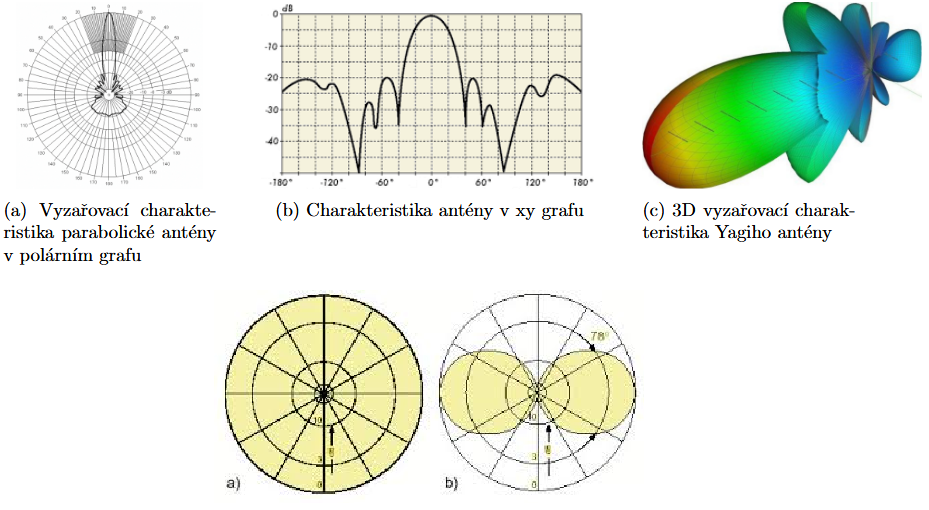
\includegraphics[width=1\linewidth]{images/image.png}
    \caption{Dipól grafy}
    \label{fig:enter-label}
\end{figure}
\newpage
\section*{5 Časté otázky ze zkouškových písemek}

\begin{itemize}
  \item Vlnová impedance – definice
  \item Vlnová impedance – určení z vlastností prostředí
  \item Vzorec pro výpočet hloubky vniku vlny do dobrého vodiče
  \item Snellův zákon lomu
  \item Co je to mezní úhel a jak závisí na permitivitě při odrazu vlny na rozhraní dvou dielektrik
  \item Na rozhraní prostředí s permitivitami $\varepsilon_1 > \varepsilon_2$ dochází k totálnímu odrazu elektromagnetické vlny. Zakreslete plochy konstantní fáze a konstantní amplitudy pro vlny na obou stranách rozhraní
  \item Uveďte vztah pro výpočet charakteristické impedance (bezeztrátového) koaxiálního vedení
  \item Uveďte vztah pro maximální střední časovou hodnotu výkonu přenášeného vlnovodem s kovovými stěnami obdélníkového průřezu s rozměry $a \times b$ při elektrické pevnosti dielektrika $E_\mathrm{max}$
  \item Vzorec pro určení vlnové délky dominantního módu vlnovodu s kovovými stěnami obdélníkového průřezu s delší stranou $a$
  \item Vyzařovací charakteristika elementárního dipólu
  \item Vztah pro určení rezonančních frekvencí dutinového rezonátoru ve tvaru kvádru s kovovými stěnami a vnitřními rozměry $a \times b \times c$
\end{itemize}
\newpage
\begingroup
\section*{6 Užitečné vzorce}

\raggedbottom
\begin{multicols}{2}
\subsection*{6.1 Kolmý dopad na rozhraní}
\[
R = \frac{Z_2 - Z_1}{Z_2 + Z_1} = \frac{\sqrt{\varepsilon_{r1}} - \sqrt{\varepsilon_{r2}}}{\sqrt{\varepsilon_{r1}} + \sqrt{\varepsilon_{r2}}}$$$$ \quad T = \frac{2Z_2}{Z_1 + Z_2} = \frac{2\sqrt{\varepsilon_{r1}}}{\sqrt{\varepsilon_{r1}} + \sqrt{\varepsilon_{r2}}}
\]
\[
Z_1 = 120\pi \sqrt{\varepsilon_{r1}}, \quad Z_2 = 120\pi \sqrt{\varepsilon_{r2}}
\]
\textbf{Pole:} $$E_{\mathrm{Rm}} = E_{\mathrm{Im}}|R|$$ $$E_{\mathrm{Tm}} = E_{\mathrm{Im}}|T|$$ $$H_{\mathrm{Im}} = \frac{E_{\mathrm{Im}}}{|Z_1|}$$ $$H_{\mathrm{Rm}} = \frac{E_{\mathrm{Rm}}}{|Z_1|}$$ $$H_{\mathrm{Tm}} = \frac{E_{\mathrm{Tm}}}{|Z_2|}$$ 
\textbf{Výkon:} $$S = \frac{1}{2} E H = \frac{1}{2} \frac{E^2}{|Z|}$$
\textbf{PSV:} $$\frac{1 + |R|}{1 - |R|}$$

\subsection*{6.2 Obecný dopad vlny na rozhraní}
\textbf{Brewsterův úhel:} $$\vartheta_\mathrm{BR} = \arcsin\left( \frac{\sqrt{\varepsilon_{r2}}}{\sqrt{\varepsilon_{r1} + \varepsilon_{r2}}} \right)$$  
\textbf{Kritický úhel:} $$\vartheta_\mathrm{krit} = \arcsin\left( \frac{\sqrt{\varepsilon_{r2}}}{\sqrt{\varepsilon_{r1}}} \right)$$  
\textbf{Vlnové číslo:} $$k_2 = \frac{\omega}{c} \sqrt{\varepsilon_{r2}}, \quad k_x = k_1 \sin \vartheta_I$$  
\textbf{Útlum (evanescentní vlna):} $$\gamma = \sqrt{k_x^2 - k_2^2}$$  
\textbf{Exponenciální pokles:} $$e^{-\gamma z}$$ – $\gamma$ je imaginární složka $k_z$

\subsection*{6.3 Parametry vlny}
$$\lambda_0 = \frac{1}{36\pi \cdot 10^9} \ \mathrm{F/m}, \quad \mu_0 = 4\pi \cdot 10^{-7} \ \mathrm{H/m}$$
$$E_x(z,t) = E_m e^{-\alpha z} \sin(\omega t - \beta z + \varphi_0)$$  
$$H_y(z,t) = H_m e^{-\alpha z} \sin(\omega t - \beta z - \varphi_z + \varphi_0)$$  
$$S_{\mathrm{str}}(z) = \frac{1}{2} E_m H_m e^{-2\alpha z} \cos(\varphi_z)$$  
$$P(z) = \frac{1}{2} \sigma E_m^2 e^{-2\alpha z}$$

\subsection*{6.4 Koaxiální kabel}
$Z_0 = \frac{60}{\sqrt{\varepsilon_r}} \ln\left( \frac{b}{a} \right)$  
$L = \frac{\mu}{2\pi} \ln\left( \frac{b}{a} \right), \quad C = \frac{2\pi\varepsilon}{\ln(b/a)}$  
$P_{\mathrm{max}} = \frac{1}{2} \frac{(E_{\mathrm{max}} a \ln(b/a))^2}{Z_0}$

\subsection*{6.5 Vlnovody}
$$f_{\mathrm{krit}}(m,n) = \frac{c}{2 \sqrt{\varepsilon_r}} \sqrt{\left( \frac{m}{a} \right)^2 + \left( \frac{n}{b} \right)^2}$$  
$$k = \frac{\omega}{c} \sqrt{\varepsilon_r}, \quad k_x = \frac{m\pi}{a}, \quad k_y = \frac{n\pi}{b}, \quad k_z = \sqrt{k^2 - k_x^2 - k_y^2}$$  
$$Z_{\mathrm{TE}} = \frac{\omega\mu_0}{k_z}, \quad Z_{\mathrm{TM}} = \frac{k_z}{\omega\varepsilon}$$  
$$P = \frac{ab}{4} \frac{E_{\mathrm{max}}^2}{Z_{\mathrm{TE}}}$$

\end{multicols}

\endgroup
\end{document}